
The contribution involves background research, theoretical designs, simulations, software design and testing. The plan revolves around the concept of audio propagation, an area that the group overall was very inexperienced with. Therefore, a significant amount of time was allocated to research to familiarise the group with audio communications.   

\subsection{Background research}

The initial background research was to see how sound travelled. This is an integral part of the project, as the sound parameter determines the range and accuracy of the product. To maximise this the background research revolved around what effected the sound, how it was measured and how to maintain clear signal. \\

The two main factors of sound propagation are the Sound Pressure Level (SPL) and the frequency. The SPL describes the relative ‘loudness’ of the sound \cite{SPL}, while frequency conveys the oscillations in the sound wave. \\

SPL is one of the methods to measure sound. The others are sound intensity level and sound power level. These parameters portray the sound wave, but SPL was chosen for his project as the microphone and speaker specifications are both given in SPL. SPL describes the ratio of the sound wave pressure and the ambient pressure that the wave is travelling through. The average variation caused by the sound wave in the atmosphere. Their relationship can be described by the equation below,

\begin{equation}
SPL = 20\log_{10}\left(\frac{p}{p_{ref}}\right) 
\end{equation}

Where \( p\) is the pressure of the sound wave, and \( p_{ref}\) is the atmospheric pressure. The SPL is used instead of the pure pressure value due to the scale of sound pressure. For example, a sound pressure of 63.2 micro Pascals is equivalent to 10dB, but a 100-dB measurement is 2 Pascals. Due to this wide range of values that produce audible sound, a logarithmic ratio is used to describe sound loudness.\\

On the surface, the frequency of the wave simply affects the pitch of the sound heard. The audible sound ranges from 20 Hz to 20 kHz  \cite{neuroscience}. Beyond those, the human ear cannot pick anything up. But this doesn't apply to speakers and microphones. Digital and analogue devices can produce and receive sound beyond human hearing range, and they do this due to the other effects frequency has on the sound. \\

Interference is the interaction of two or more waves. Interference can be either in-phase or out of phase, and it can be either destructive or constructive. The figure \ref{fig:visualisation_interference_phase_and_inphase} below illustrates this visually. 

\begin{figure}[H]
\centering
\noindent 
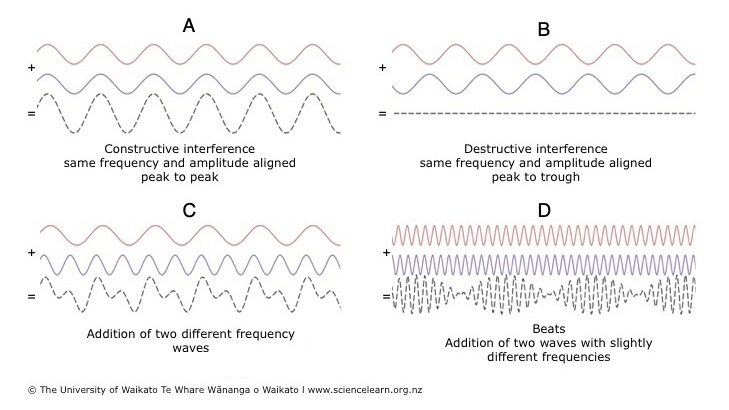
\includegraphics[width=12cm,height=6.0cm]{./images/noiseIntersaction}
\caption{Visualisation of interference in out of phase and in-phase waves \cite{noiseInt}}
\label{fig:visualisation_interference_phase_and_inphase}
\end{figure}

In the case of A, the signals are in-phase, i.e. they have the same frequency and amplitudes match, and as such, the peaks and troughs of the signal match up and result in constructive interference, as seen but the dotted line output. The signal amplitude here has essentially doubled. Conversely, in B, the signals still have the same frequency, but they do not have matched amplitudes, and as such destructive interference occurs, the amplitudes cancel out. The focus of this project will be more on cases C and D. C and D focus on variations in frequency. When two different frequencies interact, the resultant signal is a ‘noisy’ signal. This signal is distorted in amplitude and, as such harder to detect.\\ 

This initial background research defined how sound was measured, how interference can change it, and defined the important parameters that must be investigated further, SPL and frequency. 

\subsection{Work Undertaken}

The work undertaken revolves around further research, making a hypothesis on the frequency required for the project, testing, and then gaining valuable conclusion from it. 

\subsubsection{Research}

The research focused on factors affecting the SPL of the sound. These included the sound emission at the source, the loss of sound as it travels, and the noise that may affect the sound.

\paragraph{Sound Emission}

The SPL output of the speaker is determined by the frequency. Every speaker has a frequency response, meaning it can propagate specific frequencies better than others. The frequency response for the given speaker can be seen below in figure \ref{fig:speakerFR}. 

\begin{figure}[H]
\centering
\noindent 
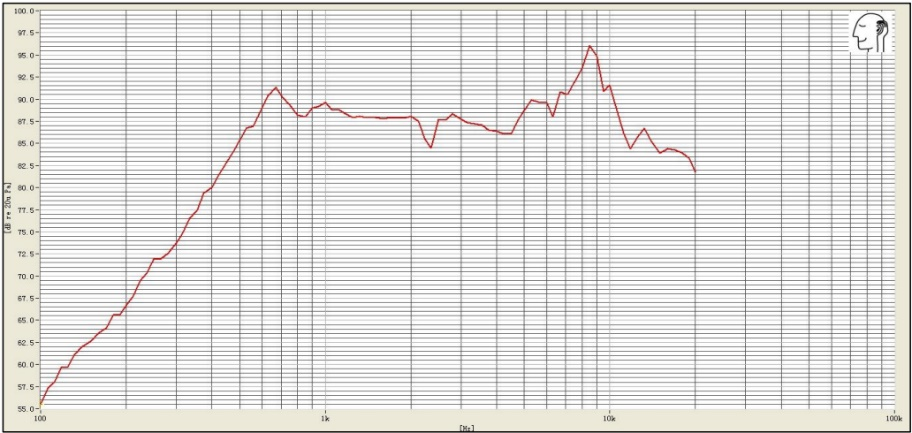
\includegraphics[width=11cm,height=6cm]{./images/image3}
\caption{Speaker Frequency Response \cite{speakerDatasheet}}
\label{fig:speakerFR}
\end{figure}

The frequency response above 1 kHz is 90+ dB for the given speaker, while at lower frequencies, it can even drop to 55dB. This is very important as, on the other side microphones have sensitivity, i.e. they require a certain level of sound to receive the signal accurately. Therefore, the higher SPL is better, and as frequency determines this, the frequency is the most significant decision that must be made in the sound area. \\

To maximise the SPL transmitted, the effect of the channel must be considered. When sound is emitted, it is subjected to attenuation and noise, both factors that result in loss and distortion. Which ultimately results in lower reliability and range.

\paragraph{Attenuation}

Attenuation is the loss of sound energy as the wave travels. The absorption of the sound wave can cause this by the air and any objects the wave interacts with. \\

Attenuation over distance follows the inverse square law. This stipulates that a point source emits a sound wave spherically, which diminishes over distance. This relationship can be described mathematically by the following 

\begin{equation}
SPL_{2} = SPL_{1}-20\log_{10}\left(\frac{R_{2}}{R_{1}}\right)
\end{equation}


Where \( SPL_{1}\) is the SPL at a distance \( R_{1}\), and \( SPL_{2}\) is the SPL at distance \( R_{2}\)  \cite{invLaw}. Through this equation, the loss of SPL purely due to distance travelled can be computed. It is frequency independent. The frequency component of attenuation only becomes relevant at extremely high frequencies. \cite{int93}. \\

Finally, there is absorption due to materials. This is measured using the absorption coefficient, which is the percentage of sound absorbed by material on a scale of 0 to 1, 1 being complete absorption. There are two types of materials commonly present in office environments, porous and reflective. Porous absorbers are materials that allow airflow, which lets the sound enter the material and dissipate as heat. These are the materials generally used in sound-proofing, as they prevent the transmission of sound. Some examples are carpet, curtains, plaster and ceiling tiles. These are commonly found materials in offices as most of them are made to reduce noise. \\

In contrast, reflective materials are generally hard, don’t allow airflow, and minimal sound enters the material. Most of the sound is reflected, and little is absorbed. Typical materials of this type are plywood, glass, and screens.  \cite{soundAtt}. \\

Each type of material reacts differently to frequency. Below in figure \ref{fig:matAtt}, an example of this can be seen. 

\begin{figure}[H]
\centering
\noindent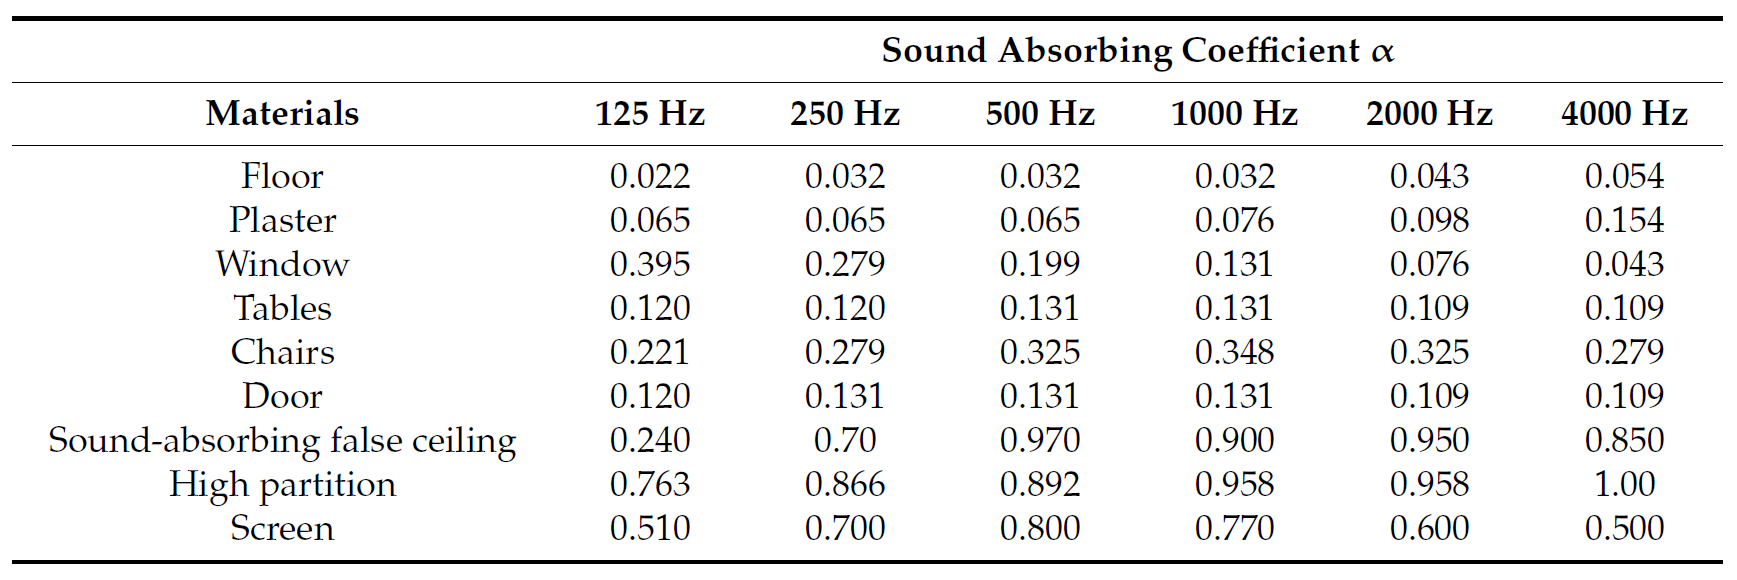
\includegraphics[width=13.48cm,height=4.5cm]{./images/matAtt.png}
\caption{Sound absorption Coefficients of Various Materials. \cite{openPlan}}
\label{fig:matAtt}
\end{figure}

The reflective materials tend to attenuate lower frequency sound better, while porous  materials attenuate higher frequencies better. For example, plaster, a porous material, has an absorption coefficient of 0.154 at 4 kHz, while only has a 0.065 coefficient at 125 Hz. Conversely, a hard-reflective material like a window has a coefficient of 0.043 at 4 kHz, while at 125 Hz, it has a coefficient of almost 0.4. This illustrates that the chosen frequency will also determine the attenuation loss via objects within the office. \\

The change in frequency also affects attenuation due to temperature and humidity, due to how air particles are affected. Increases in temperature and humidity result in less attenuation. Still, these factors were not heavily investigated, as the temperature and humidity of the target environment are regulated and not a variable. \\

In summary, the attenuation of travelling sound is greatly affected by frequency and initial sound pressure. To maximise both, the correct frequency must be chosen. 

\paragraph{Noise}

Noise is the interference of outside sound sources, corrupting the transmitted signal. The interference of the signal can cause it to lose SPL and be less detectable at the microphone. The main aim of noise investigation is to find common noise sources in an office and what common frequencies are present. This is important so that the chosen frequency is not one that is commonly found in the target environment, and as such, can be easily filtered for without being corrupted. The distribution of noise in an average office can be seen in the figure \ref{fig:noise} below. 

\begin{figure}[H]
\centering
\noindent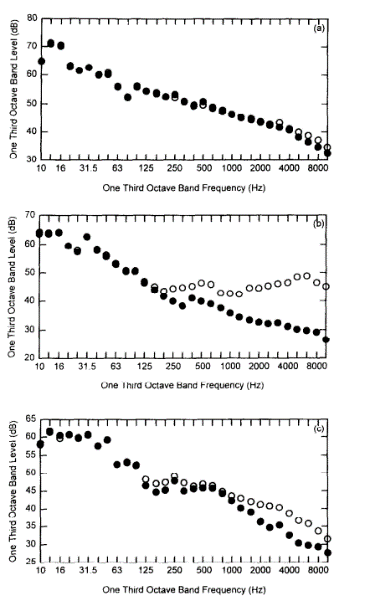
\includegraphics[width=5.57cm,height=9.0cm]{./images/noise.png}
\caption{Ambient Sound levels in various offices \cite{noiseRep}}
\label{fig:noise}
\end{figure}

The figure describes the ambient noise level at different frequencies in 3 various offices. More noise is present at frequencies lower than 1600 Hz, particularly in the sub 250 Hz range. This information is factored into the frequency decision, as ambient noise frequencies with high SPL will interfere with similar frequencies signals and cause loss. 

\subsubsection{Simulations}

Simulations were conducted to gain a better understanding of how the sound changed as it travels. All Simulations are included in the Appendix A. \\

The first simulation was to determine the max transmission distance with the current equipment in an undisturbed channel, i.e. no noise or attenuation other than distance. Equation 2 was used to simulate this on MATLAB. The \( R_{1}\) measurement was at 10cm and the \( SPL_{1}\) was 90dB for the theoretical 1 kHz frequency being delivered, found on the frequency response of the speaker. The lowest detectable sound for the microphone can be found by examining its datasheet. The SNR is the difference in decibels between the noise level and the reference signal (1 kHz). The microphone does not produce an output if any input signals are below the noise floor, which is defined by the following relationship 

\begin{equation}
noise floor = SPL_{ref}-SNR
\end{equation}

By calculating both parameters and graphing them, the intersection will illustrate the max free communication distance. The simulation can be seen in Appendix A. \\

The calculated noise floor of the microphone was calculated to be 28.5 dB, as indicated by the black line on the figure above. The SPL of the sound falls away as distance increases and interacts with this line at 120m. this is the approximate, max unobstructed communication distance for sound at 1 kHz. \\

Investigating the effect of rising frequency on the air absorption attenuation ISO standard 9613-1  \cite{int93} was used to value dB loss over distance. These were plotted in Appendix A. \\

The attenuation via air increases as the frequency increases, but even at very high frequencies, the loss I relatively small, not even more than 1 dB. This illustrates that the air absorption due to frequency is minimal and that this limitation can be ignored or given less weighting when deciding the output frequency. \\

Simulations for the attenuation of the conflicting material types, reflective and absorptive were made, to illustrate their differences. The comparison of carpet and plywood can be seen below in Appendix A. \\ 

The opposing trends visualise the difference. One falls as frequency rises while the other rises with it. There is a balance point at 1000 Hz wherein both attenuation coefficients are of comparable values at 0.1. In future simulations, all common materials can be simulated to find common issues where attenuation can be equally minimised.

\subsubsection{Theoretical design}

Collating all this this theoretical information, a visual diagram was formed to illustrate where the best available frequencies for transmission are. This can be seen in figure \ref{fig:gZone}. 

\begin{figure}[H]
\centering
\noindent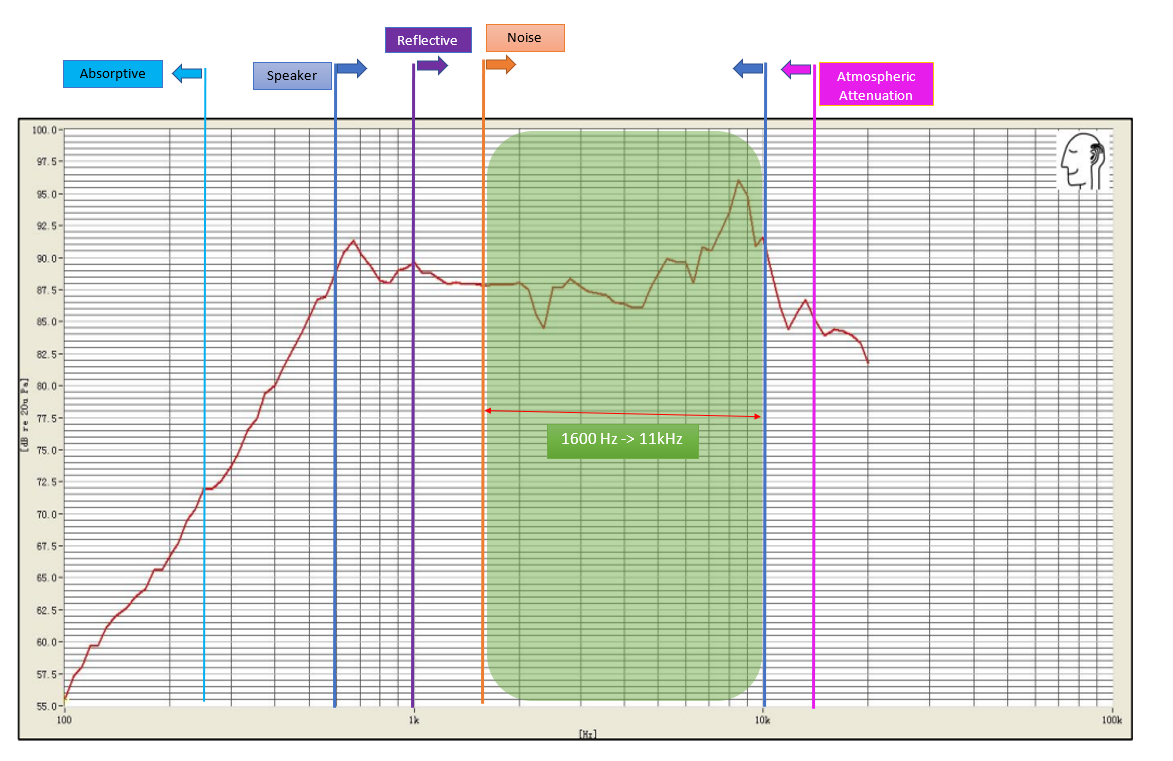
\includegraphics[width=16.64cm,height=9.5cm]{./images/greenZone.png}
\caption{Green Zone Diagram}
\label{fig:gZone}
\end{figure}

The green zone diagram illustrates how the limiting factors affect the choice of frequency. It is overlaid upon the speaker’s frequency response to further illustrate which frequencies within the green zone would be effective. A table is include in Appendix B to illustrate the exact bounds. The main concerns now are the attenuation factors due to materials, as they are the most significant constraints. Noticeably there is one bound that cannot be fulfilled. The absorptive (porous) material bound is simply too low for most speakers, and is unlikely to be fulfilled regardless of the apparatus used. To verify the green zone testing was undertaken, using the microphone/speaker system. 

\subsubsection{Software design and Test}

When testing was due to be done there was no reliable microphone code that could be used to verify the received sound. This meant there was no way to compare the effect of various frequencies on the reception. So, to complete testing some software must be designed for the microphone. The majority of the software design surrounding the microphone will be covered in other sections, this section is specifically software designed for testing purposes. \\

Initially, there was no way of seeing the output from the microphone as a waveform output. Only sound level could be seen, and even then, on a very small, sensitive scale. It used the \textit{rms }function which modelled the microphone output on a scale of 0.0 to 1.0. On this scale the difference between ambient and a received signal was 0.0005, and this was only at a maximum of 8cm away. This was an unacceptable and incorrect result and it was clear the microphone needed a better software implementation. To achieve this the \textit{queue }functionality was explored. \\

The \textit{queue }function solved a key problem in the printing of the microphone output. The microphone was being sampled at 44 kHz, and due to the limitations of the serial monitors of the Arduino IDE software, the sampling rate was too fast for the output. The Arduino IDE’s maximum serial output rate is 115200 bits/sec \cite{arduino}The output of the microphone is stored as a 32-bit floating-point value, and so the effective sample output rate becomes 115200/32, which is far lower than the nominal input and such cannot be output one to one. As such it must be stored in a buffer and output at a slower rate. Luckily there was a \textit{queue} function which enabled exactly this functionality. \\

The \textit{queue} function stores 128 samples which can be copied to a buffer periodically, and then printed. Essentially the \textit{queue} begins and data is stored, once the queue is full the data is printed. An overview for this piece of code can be seen in figure \ref{fig:qFlow} 

\begin{figure}[H]
\centering
\noindent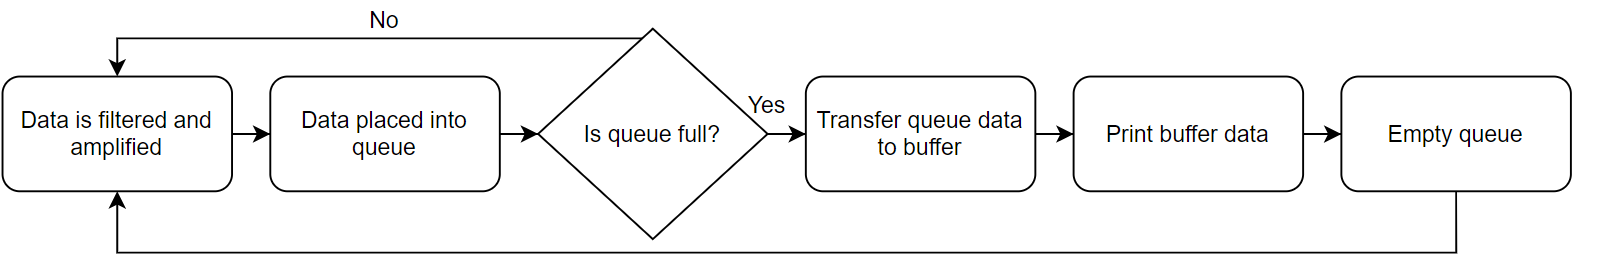
\includegraphics[width=18cm,height=3.0cm]{./images/queueFlowH.png}
\caption{Flowchart Overview of Testing Code}
\label{fig:qFlow}
\end{figure}

The initial filtering is used to remove any noise components in the received data, and this is amplified to reasonable output level. The filter and amplification processes will be described further in later sections. The printed output of the buffer can be seen in figure \ref{fig:qOut}. 

\begin{figure}[H]
\centering
\noindent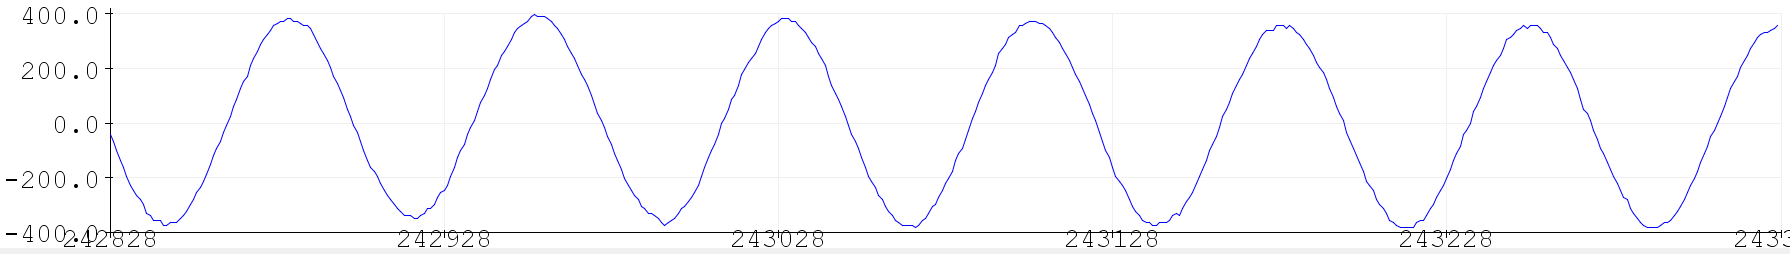
\includegraphics[width=15.92cm,height=2.27cm]{./images/queueOutput.png}
\caption{Output of Test Code}
\label{fig:qOut}
\end{figure}

The input for this output was 1 kHz signal at a 20 cm range. This clearly verifies the performance of the microphone and illustrates that data can be read and seen from it. This will be essential in later stages where the waveform will need to be processed. 

\subsubsection{Test section}

Testing was completed inside a student work shop room. The room is by no means designed for sound testing, but due to the circumstances it was the best available space. The room had an empty middle space, upon which a desk was place and testing was conducted. This was to reduce the effect of reflection. In another effort to minimize reflection the tests wee taken over a small distance of 1m. This was to guarantee good reception, as the maximum distance was not the factor being tested. The speaker and microphone were placed at 1m distance on a level plane. This provided the system with the best possible conditions for transmission. Frequencies were swept from 1 kHz to 15 kHz in steps of 1 kHz, and the output was examined. Maximum amplitude for each frequency was recorded and graphed in \ref{fig:testResult}

\begin{figure}[H]
\centering
\noindent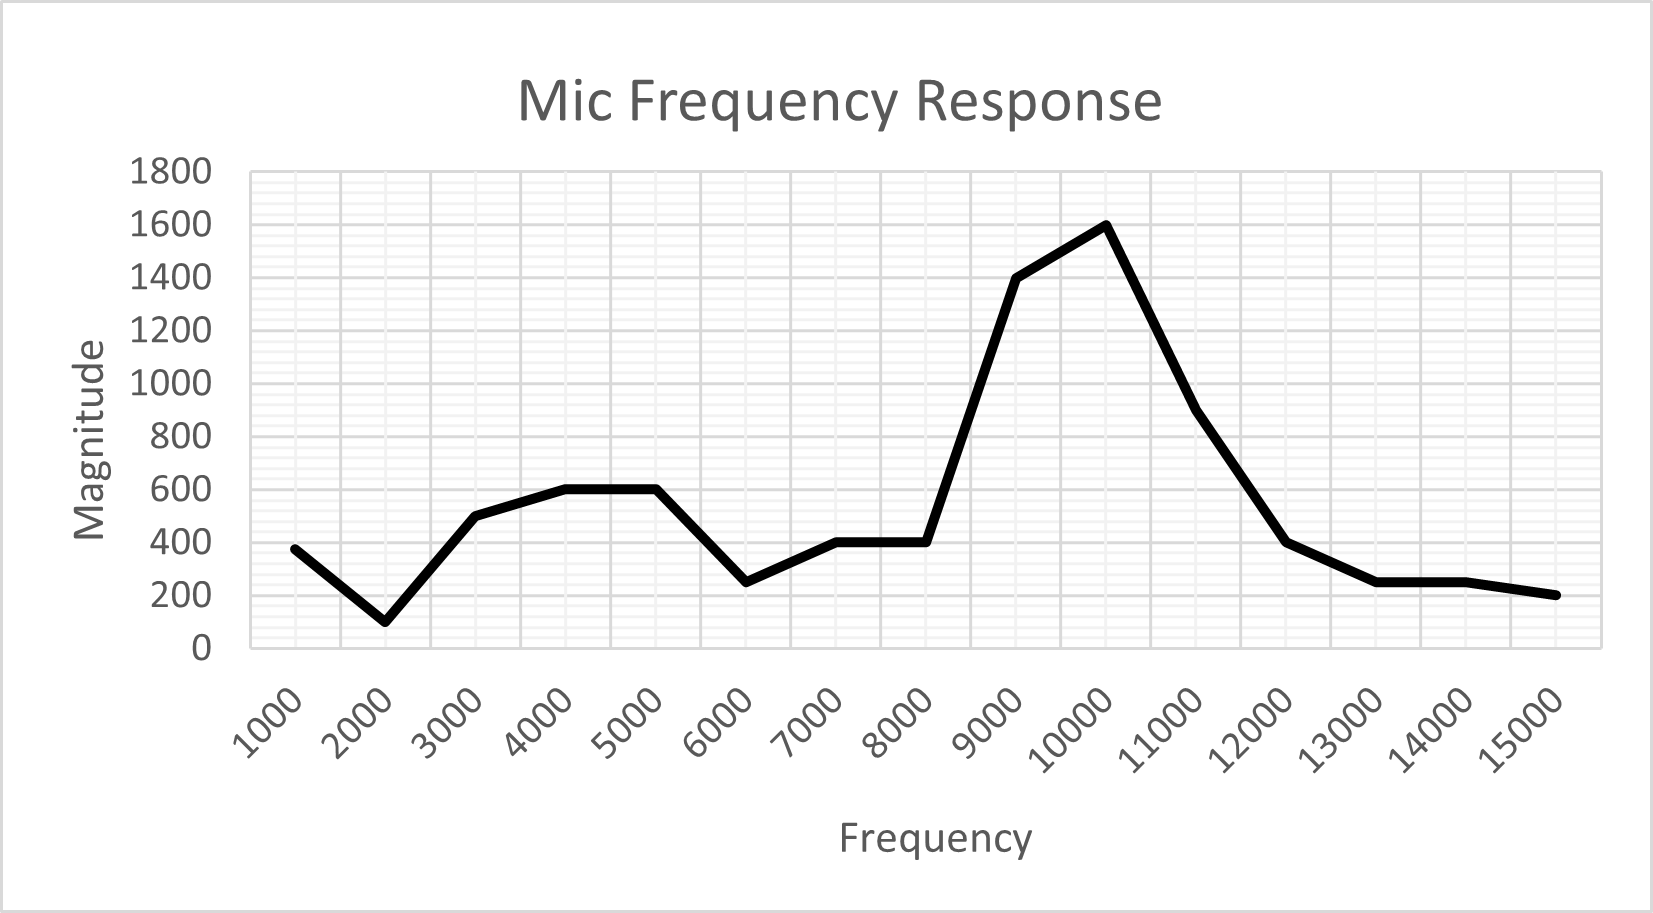
\includegraphics[width=13.53cm,height=7cm]{./images/testResult.png}
\caption{Test Setup}
\label{fig:testResult}
\end{figure}

The results verify the hypothesis as the they follow the speaker’s frequency response. There is a considerable rise at 9 kHz – 10 kHz and then drop off at 11 kHz, as seen in figure \ref{fig:speakerFR} \\

The second test was to verify the maximum distance of communication. The set up for this was in a long narrow corridor with the microphone and speaker again on an even plane. Tests were conducted using the 10 kHz frequency, as this was the best one from the past test. \\

This resulted in a maximum distance to be at 18m (without filtering). When a high pass filter was added for a 10 kHz cut-off this distance increased to 24m. Beyond these points the reception would distort or the magnitude of the signal would fall below the noise. The signal shape and magnitude must be maintained for it to be processed further, via either convolution or peak detection (described in further sections). 

\subsection{Discussion}

In accordance with the requirements the sound transmitted must be robust to noise and be able to accurately produce a distance calculation. For both requirements to be fulfilled, the sound must maintain a high SPL. The most important factor affecting the level of sound is the frequency of it. The frequency defines almost all the loss components involved in the signal transmission. Through testing and research conducted the best way to mitigate the loss of SPL is to pick an ideal frequency range which will be least affected by these factors. \\

Using said research a hypothesis was created in the form of the green zone diagram in \ref{fig:gZone}. This diagram stipulated that to avoid unwanted factors like noise, attenuation, and sub-par hardware performance the frequency chosen must be with the 1600 Hz to 11 kHz range. This hypothesis was then tested and confirmed. The best frequency range found was between 9 kHz and 10 kHz. \\

This raises some considerations. The sound played, if chosen to be between 9 kHz and 10 kHz will be resilient to almost all factors except porous materials. The absorption for porous materials scales greatly as the frequency rises. This is unfortunate as modern offices are filled with porous materials. For example, carpets, spongy soundproofing barriers and drapes are all examples of absorptive materials. Due to their abundance in the workplace a frequency like 10 kHz may be easily absorbed and unsuccessfully transmitted. \\

With the current implementation choices, i.e., hardware, audible sound, the problem of porous materials is very hard to mitigate. This is due to the very low frequencies required for low absorption, almost at less than 250 Hz. This causes two problems, firstly there are not any speakers of the size Wellnomics are investigating that can produce such low frequencies, and this low frequency will be easily absorbed via reflective materials present in the work environment. As such the research completed indicates that a frequency must be picked to balance the absorption of the two material types, absorptive and reflective. Even if this frequency is not ideal to the hardware used it can still be more effective than the preferred 10 kHz frequency. \\

As such a lower frequency, like 1.6 kHz - 2 kHz may be preferable. Even though this does not provide the absolute best speaker performance, as seen in figure \ref{fig:testResult}, it is the lowest frequency which the absorption co-efficient for most porous materials is still less than 0.3 \cite{jwc}. This frequency still lies with in the green zone, and as such still fulfils the other constraints. The conclusion from this is that even though the 10kHz is the best performing frequency for the system, this may nt be true in practice due to material attenuation. \\

The noise in offices is often low frequency, as seen in \ref{fig:noise} and as such needs to be accounted for. But if measurements were taken outside of office hours or not in the presence of employees, then the noise factor can be largely ignored, leading to a greater spectrum of options. The 1 kHz to 1.6 kHz range becomes viable if measurements are taken in the absence of noise. This range is again more suitable for porous  materials while still providing for the hardware and reflective requirements. \\

In conclusion it is evident from the research and testing that that there are many important factors which contribute to the sound level, but paramount among them is the attenuation via materials. As these will act as barriers and absorb the sound. So, it is important not only examine the microphone performance and noise, but to be weary of how frequency will interact with the two material types. I believe a lower frequency such as 1 kHz – 2 kHz could potentially be used in the absence of noise, or a higher frequency can be used in the absence of porous materials. Table \ref{tab:Final choice} describes the final frequency ranging choices.

\begin{table}[H]
\captionsetup{singlelinecheck = false, format= hang, justification=raggedright, font=footnotesize, labelsep=space}
\caption{Final Frequency Choices}
\begin{adjustbox}{max width=\textwidth}
\begin{tabular}{p{7.95cm}p{7.95cm}}
\hline
\multicolumn{1}{|p{7.95cm}}{Scenario } & 
\multicolumn{1}{|p{7.95cm}|}{Frequency Range} \\ 
\hline
\multicolumn{1}{|p{7.95cm}}{Absence of Porous materials } & 
\multicolumn{1}{|p{7.95cm}|}{9 kHz – 10 kHz} \\ 
\hline
\multicolumn{1}{|p{7.95cm}}{Presence of Porous materials } & 
\multicolumn{1}{|p{7.95cm}|}{1.8 kHz - 2 kHz} \\ 
\hline
\multicolumn{1}{|p{7.95cm}}{Presence of Porous materials, Absence of Noise } & 
\multicolumn{1}{|p{7.95cm}|}{1 kHz - 2 kHz} \\ 
\hline
\end{tabular}
\end{adjustbox}
\label{tab:Final choice}
\end{table}

The investigation into sound reveals that the target environment plays a major role, more so than the hardware and the noise present. Both the hardware and the noise can be mitigated via other methods, like changing to a microphone which works better in lower frequencies, or by conducting distance measurements in quieter times. But the material environment is out of the control of the manufacturer. Wellnomics could consider an adaptive approach wherein all three cases are accounted for and based on the environment, the sent signal's frequency is changed. To best prepare for any environment the suggestion is to use the "Prescence of Porous Materials" case and choose a frequency of $\sim$1.8 kHz for distance measurement. This may be the most reliable frequency when considering the hardware, noise and most importantly attenuation factors present. With these choices the design fulfils the desired requirements for the project. \\



